\section{문제 정의와 제안 방법}\label{sec:method}
\subsection{시스템 입력과 기반 추정기의 역할}

전체 시스템은 RGB(Red, Green, Blue) 컬러 영상 $I$, 카메라 내부파라미터 $\K$, 팔레트의 가로·깊이·높이 $\dvec=(W,D,H)$를 입력으로 사용한다. 자세는 카메라에 대한 회전 $\R\in SO(3)$과 위치 $\tvec\in\mathbb R^3$으로 정의한다. \textbf{초기 추정기는 영상에서 코너와 특징을 추출하고, 제안 보정 신경망은 이 결과와 물리적 치수를 함께 입력받아 코너를 수정한다.} 같은 치수는 최종 자세 계산에도 사용된다.

기반 추정기를 $f_{\theta_\beta}$, 기반별 특징·출력 연결부를 $h_\beta$로 나타낸다. 연결부는 각 추정기의 출력을 초기 코너 8점·중심점 1점, 유효성 마스크, 박스와 두 수준의 특징으로 변환한다. 보정기를 학습하는 동안 초기 추정기의 가중치는 고정한다. 본문의 모든 Base는 제공된 치수 숫자를 초기 코너 산출에 직접 입력하지 않는 RGB 모델이며, 합성 감독으로 학습한 보정기가 치수를 추가 활용한다. 별도로 존재하는 ResNet 직접 치수 입력 FULL 모델은 이 연구의 Base가 아니다.

YOLO는 검출기 고유의 박스와 점수를 사용한다. DOPE 연결부는 유효 예측 코너의 범위에서 박스를 만들고 코너 확률맵의 최대값을 점수로 사용한다. 원래 DOPE의 affinity 기반 다중 객체 연결과 다른 디코딩 경로이므로, 이 점수를 YOLO 검출 신뢰도와 동등하게 취급하지 않는다. ResNet-18 몸체는 잔차 신경망 원전\cite{resnet2016}에, 세 개의 256채널 역합성곱과 마지막 9채널 확률맵 헤드는 Simple Baselines for Human Pose Estimation and Tracking\cite{simple2018}의 구조에 근거한다. 전체 영상·팔레트 9점·분포 기댓값 디코더는 이 저장소의 변형이며 원 인체 벤치마크 재현이 아니다. 이 기반은 치수 문맥을 0으로 고정하여 합성 자료로 10 epoch 학습한 CONSTANT 기반이다. 그 고정 특징 변환을 마지막 합성곱에 합쳐 RGB만 입력받게 하며, 공간 확률분포의 기댓값으로 초기 좌표를 계산한다. CONSTANT는 치수 조건이 고정되었다는 뜻으로, 이미지에 따른 좌표 출력이 상수라는 뜻이 아니다. 기반별 전처리·디코더·특징 연결의 상세는 보충자료에 정리한다.

보정 대상은 코너 $k=0,\ldots,7$이다. 객체 선택, 박스, 점수, 후보 순서, 중심점 $k=8$ 및 결측 마스크는 변경하지 않는다. 이 출력 보존은 코너나 자세 정확도의 보존을 보장하지 않는다. 치수는 등록된 객체 정보에서 제공하며 영상으로 임의 팔레트의 규격을 추정하지 않는다.

\begin{figure*}[t]
\centering
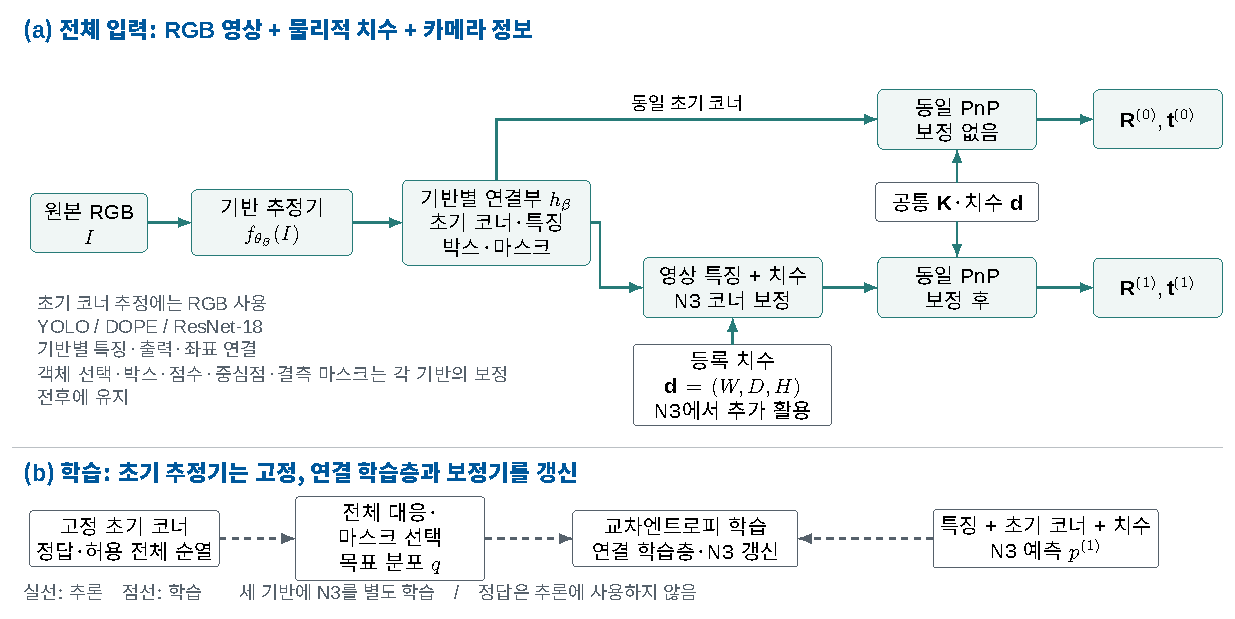
\includegraphics[width=.98\textwidth]{figures/process_overview.pdf}
\caption{제안 시스템의 입력과 보정 전후 경로. 초기 RGB 추정기의 동일 출력에서 출발하며 제안 보정기는 영상 특징·초기 코너·물리적 치수를 함께 사용한다. Base와 보정 후 경로의 자세 계산에는 같은 카메라 정보와 치수가 제공된다. 실선은 추론, 점선은 합성 정답에 의한 보정기 학습이다.}\label{fig:pipeline}
\end{figure*}

\subsection{좌표계와 기반별 특징 연결부}
원본 영상 좌표를 $\uvec^I$, 기반 $\beta$의 네트워크 입력 좌표를 $\uvec^{N,\beta}$로 구분한다. 크기 변환과 패딩의 관계는 다음과 같다.
\begin{equation}
 \uvec^{N,\beta}=A_\beta\uvec^I+\mathbf a_\beta,
 \quad A_\beta=\operatorname{diag}(g_{x,\beta},g_{y,\beta}).
 \label{eq:affine}
\end{equation}
여기서 $\mathbf a_\beta$는 패딩 등에 의한 평행이동이다. 이동 벡터의 역변환에는 평행이동이 포함되지 않는다. 이미지, 코너, 박스와 특징 표본 위치는 같은 전처리 기록을 사용한다. YOLO에서 하나의 크기 비율을 쓰는 경우와, 실제 가로·세로 크기로 축별 비율을 계산하는 DOPE·ResNet 연결을 구분한다.

두 특징을 $F^{(1)}_\beta,F^{(2)}_\beta$로 쓴다. 기반마다 채널 수와 특징 간격이 달라 연결층을 별도로 학습한다. 후보 구성·치수 표현·분포 계산·이동 상한은 공통이며, 특징 셀 중심에 따른 보간 규칙과 원본 좌표 변환을 기반별로 적용한다.

\subsection{국소 후보와 시각적 점수}
이 절의 박스와 좌표는 네트워크 입력 기준이다. 예측 박스의 대각선을 $\ell_\beta^N$라 하면, 각 코너의 이동 후보는 13개 방향과 17개 반경으로 구성된다. 정규화 변위 $\vvec_j$의 최대 노름은 0.08이고, 영벡터 후보를 추가해 총 $J=222$개를 사용한다.
\begin{equation}
 \uvec_{kj}^{N,\mathrm{cand}}=\uvec_k^{N,\beta}+\ell_\beta^N\vvec_j,
 \qquad \vvec_J=\mathbf0.
 \label{eq:candidate}
\end{equation}
221개 이동 후보 주변의 $4\times8$ 격자에서 두 수준의 특징을 보간하고 결합한다. 학습 가능한 $1\times1$ 채널 변환과 공유 패치 인코더를 거친 평균·최대 집계에 코너 역할, 박스 내 위치 및 후보 이동 정보를 결합하여 후보 점수를 얻는다. 무이동 후보는 동일한 패치를 하나 더 추출하는 대신, 후보 특징의 집계와 코너 맥락을 읽는 별도 점수 분기를 사용한다. 이들을 합친 시각 점수를 $z^{\mathrm{vis}}_{kj}$로 표시한다.

\subsection{치수 정보에 의한 후보 점수 조정}
미터 단위의 치수에서 다음 5차원 특징을 구성한다. 로그 길이는 1m를 기준으로 한 수치이며, 표준화의 평균·표준편차는 학습 자료에서 고정한다.
\begin{equation}
 \mathbf c(\dvec)=\left[\log W,\log D,\log H,
 \log\frac{W}{D},\log\frac{H}{\sqrt{WD}}\right].
\end{equation}
치수 인코더는 5차원 입력을 16차원으로 변환한다. 여기에 코너 역할 8차원, 정규화 후보 변위 2차원, 무이동 표시 1차원을 결합해 27차원을 구성하고, 작은 다층 신경망으로 모든 222개 후보의 치수 점수를 계산한다.
\begin{equation}
 z_{kj}=z^{\mathrm{vis}}_{kj}+z^{\mathrm{dim}}_{kj}.
\end{equation}
치수 점수 분기의 마지막 층은 영으로 초기화한다. 치수는 후보 \emph{점수}를 조건화하며, 후보의 기하 위치를 치수로 직접 이동시키거나 가려진 코너를 해석적으로 복원하는 입력이 아니다. 추론 시 대칭 종류 코드를 별도로 입력하지 않는다. 3차원 치수와 영상상의 종횡비는 같은 값이 아니며, 시점·회전·거리의 영향으로 정사각형 물체도 영상에서는 다른 사각형으로 보일 수 있다. 따라서 치수를 이용해 영상의 코너를 정사각형으로 강제하지 않는다.

\begin{figure*}[t]
\centering
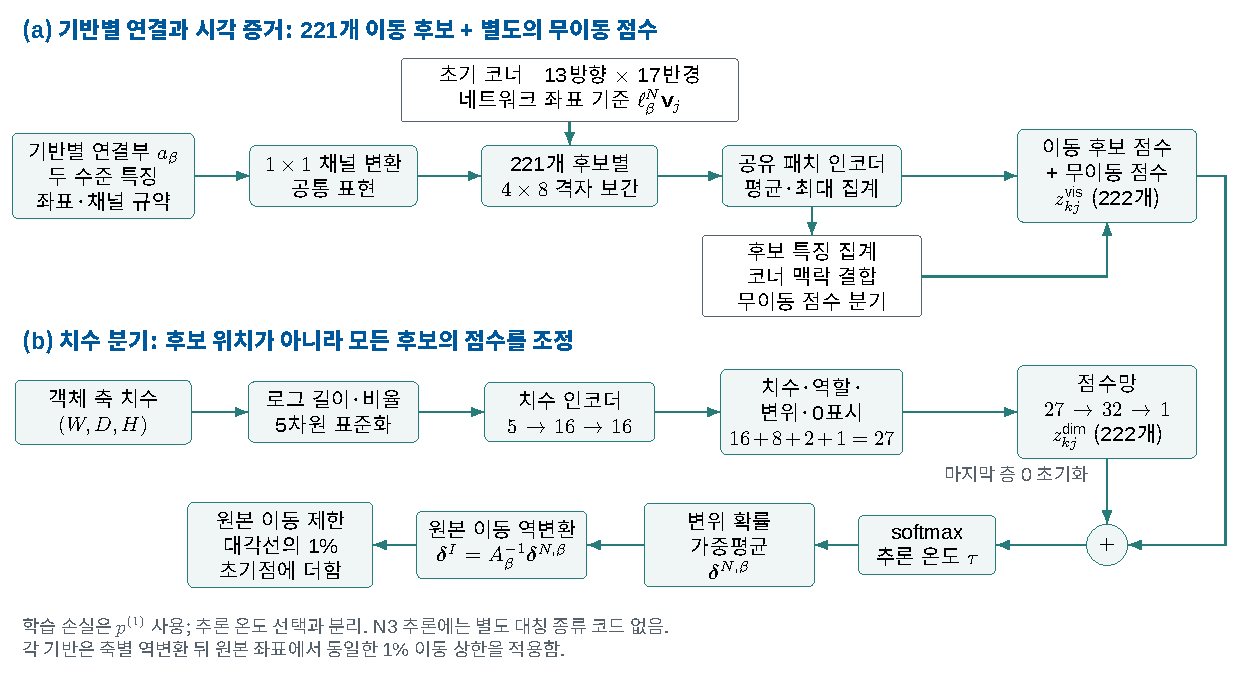
\includegraphics[width=0.97\textwidth]{figures/refiner_architecture.pdf}
\caption{국소 보정 신경망. 두 수준의 영상 특징으로 얻은 시각 점수와 치수 점수를 합하고, 이동 후보의 확률 가중평균을 원본 좌표로 복원한다. 무이동 후보의 시각 점수는 별도 집계 분기를 사용한다. 후보 점수 조정은 치수에 따른 기하 형상 강제와 다르다.}
\label{fig:architecture}
\end{figure*}

\subsection{분포 출력과 원본 좌표의 이동 제한}
추론에서는 온도 $\tau>0$를 적용한 분포의 기댓값으로 네트워크 좌표 이동을 계산한다.
\begin{align}
 p_{kj}^{(\tau)}&=\frac{\exp(z_{kj}/\tau)}{\sum_{l=1}^{J}\exp(z_{kl}/\tau)},\\
 \bm\delta_k^{N,\beta}&=\lambda\ell_\beta^N\sum_{j=1}^{J}p_{kj}^{(\tau)}\vvec_j.
 \label{eq:delta_net}
\end{align}
기댓값으로 좌표를 얻는 일반 원리는 Integral Human Pose Regression\cite{integral2018}과 관련되며, 여기서는 국소 변위 후보에 사용한다. 원본 좌표의 이동 벡터와 제한은 다음처럼 명시한다.
\begin{align}
 \bm\delta_k^I&=A_\beta^{-1}\bm\delta_k^{N,\beta},\\
 \bar{\bm\delta}_k^I&=\bm\delta_k^I\min\!\left(1,\frac{\alpha D_I}{\|\bm\delta_k^I\|_2}\right),\\
 \uvec_k^{I\prime}&=\uvec_k^I+\bar{\bm\delta}_k^I.
 \label{eq:original_cap}
\end{align}
$D_I$는 원본 영상의 대각선, $\lambda=1$, $\alpha=0.01$이다. 이동이 영벡터이면 배율은 1이다. 등방 크기 변환인 $A_\beta=gI_2$에서는 네트워크 좌표의 상한 $\alpha D_Ig$를 적용한 뒤 $g$로 나누는 것과 같다.

유효 초기점이나 특징 지원이 없는 코너는 새 좌표로 완성하지 않고 그대로 유지한다. 이동 제한은 큰 수정을 막지만 작은 잘못된 수정까지 방지하지 않는다.

\subsection{객체 전체의 회전 대응과 학습 손실}
객체 구조와 주석 규칙에서 허용하는 전체 코너 순열 집합 $\Pi_i$를 사용한다. $0^\circ$·$180^\circ$의 두 대응은 180도 회전 동등성($C_2$), $0^\circ$·$90^\circ$·$180^\circ$·$270^\circ$의 네 대응은 90도 간격 회전 동등성($C_4$)이다. 데이터 집단은 직사각형·정사각형으로 구분하되, 지지면의 형상만으로 객체나 포크 작업의 회전 동등성을 자동 결정하지 않는다. 각 순열은 코너 전체에 일관되게 적용한다.

학습에서는 \emph{고정된 초기 예측}과 허용된 정답 코너 배열 사이의 평균 정규화 거리가 작은 전체 순열 하나를 선택한다. 코너를 독립적으로 재매칭하지 않고 정답 좌표와 유효성 마스크를 같은 순열로 옮긴다. 결측 예측의 정규화 벌점은 1이며 동률은 원래 대응을 우선한다. 이 단계는 최종 보정 손실에 대한 순열별 최솟값 선택과 다르다.

선택된 정답에서 초기 예측을 뺀 네트워크 좌표 잔차를 $\mathbf r_k^{N,\beta}$라 하면, 목표 분포는 다음과 같다.
\begin{equation}
 q_{kj}=\frac{\exp[-\|\ell_\beta^N\vvec_j-\mathbf r_k^{N,\beta}\|_2^2/(2\sigma^2)]}
 {\sum_l\exp[-\|\ell_\beta^N\vvec_l-\mathbf r_k^{N,\beta}\|_2^2/(2\sigma^2)]},
 \quad \sigma=\frac{0.08\ell_\beta^N}{17}.
\end{equation}
실제 학습의 예측 분포는 $p^{(1)}$, 즉 온도 1의 softmax이다. $m_{ik}$를 해당 영상·코너의 유효 감독 표시, $n_i=\sum_km_{ik}$라 하면 손실은
\begin{equation}
 \mathcal L=\frac{\sum_i\mathbf1[n_i>0]\,
 \frac{1}{\max(1,n_i)}\sum_km_{ik}[-\sum_jq_{ikj}\log p^{(1)}_{ikj}]}
 {\max(1,\sum_i\mathbf1[n_i>0])}.
\end{equation}
학습 후 합성 보정 집합에서 선택하는 추론 온도와 학습 손실을 구분한다. 정답과 정답 기반 순열 선택은 배포 추론에 존재하지 않는다.

\begin{figure*}[t]
\centering
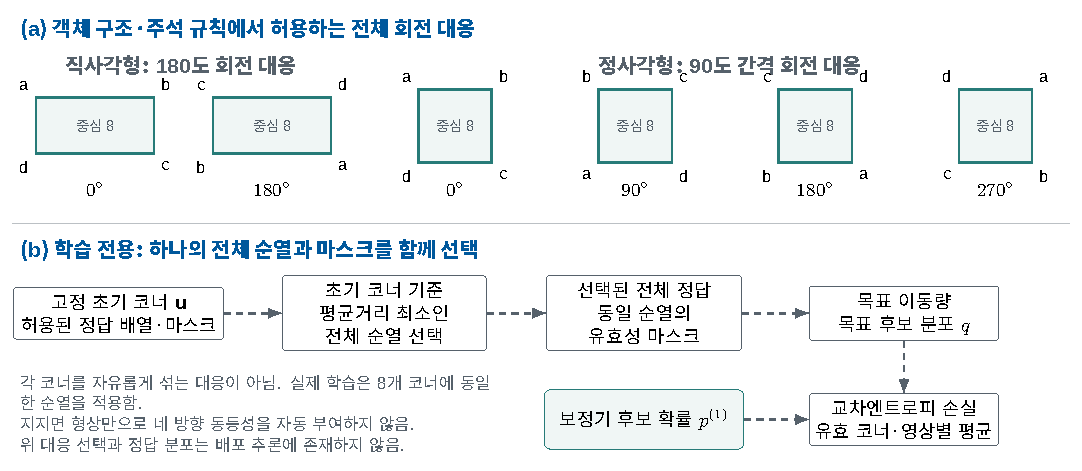
\includegraphics[width=\textwidth]{figures/symmetry_supervision.pdf}
\caption{직사각형과 정사각형의 전체 회전 대응 예시 및 학습 경로. a--d는 윗면을 설명하기 위한 표시이다. 초기 예측을 기준으로 하나의 전체 순열을 선택하고 8코너와 유효성 마스크를 함께 옮긴다. 정사각형의 네 방향 예시는 허용 가능한 대응의 설명이며, 본 합성 학습에 네 방향 대응 표본이 있었다는 뜻이 아니다. 해당 학습 행 수는 0개였다.}
\label{fig:symmetry}
\end{figure*}

\subsection{동일한 기하 계산을 통한 자세 산출}
원래 코너와 보정 코너에는 같은 Perspective-n-Point(PnP) 절차를 적용한다. PnP는 알려진 3차원 점과 영상 대응점, 카메라 내부파라미터로 위치·회전을 구하는 문제이다. \textbf{보정 없는 기준선도 같은 치수로 구성한 3차원 코너를 사용한다.} 따라서 N3의 치수 효과는 치수를 최초로 알려주는 효과가 아니라, 이미 자세 계산에 제공한 치수를 보정 점수에서도 활용하는 효과이다.

자세 계산은 예측에만 의존하는 가로·깊이 가설 선택, SQPnP\cite{sqpnp2020} 및 비선형 정밀화로 구성된다. 추정 코너가 바뀌어 선택된 가설이 달라질 수 있으나, 선택 알고리즘과 정보 조건은 고정한다. 유효 코너가 부족하거나 해가 유효하지 않으면 실패로 남긴다. 카메라·치수·객체 축·좌표 복원·실패 처리를 결과에 맞춰 변경하지 않는다.

본 평가의 $C_2$와 $C_4$는 정준 xyz=[W,H,D]의 수직 Y축을 중심으로 하는 각각 $\{0,\pi\}$와 $\{0,\pi/2,\pi,3\pi/2\}$의 허용 회전군이다. 정준 좌표의 해당 수직 축과 camera-facing 코너 순서는 저장소의 고정 축 변환에 따른다. $W=D$라는 치수 등식만으로 포크 입구, 적재물, 외관의 90도 동등성을 승인하지 않으며, 데이터의 허용 전체 대응 계약에서 선언한 순열에만 적용한다.
